\section{Introduction}
\label{sec:intro}


\section{Background}
\label{sec:background}

\subsection{RDMA}

RDMA is a networking technology which allows client machines
to directly access the memory of a remote server. RDMA is an
enabling technology for memory disaggregation as
\textit{memory servers} do not need any computation
resources (save setting up the RDMA memory initially).

One sided RDMA verbs (read, write, atomic) are used to
access remote memory without any memory side computation.
One sided verbs require RDMA reliable connections which
guarantee in-order delivery of operations.

\subsection{Resource Disaggregation}

\subsection{Cuckoo Hashing}

%%path length and locking
A colision when inserting into a cuckoo hash table requires
displacing some number of keys. The sequence of displaced
keys called a \textit{cuckoo
path}~\cite{cuckoo-improvements}.


\subsection{Remote Memory Data Structures}

\section{Problems}
\label{sec:problems}

\begin{figure*}[t]
    \centering
    \begin{subfigure}{0.3\linewidth}
        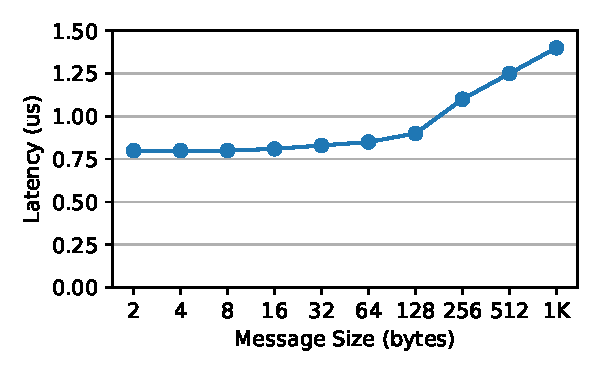
\includegraphics[width=0.99\linewidth]{fig/rdma_latency.pdf}
        \label{fig:rdma_latency}
        % \caption{}
    \end{subfigure}.
    \begin{subfigure}{0.3\linewidth}
        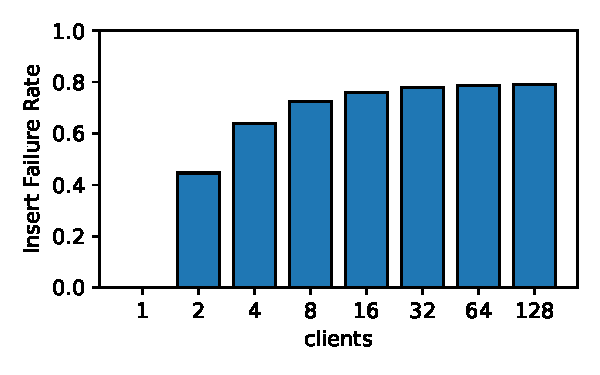
\includegraphics[width=0.99\linewidth]{fig/optimistic_failures.pdf}
        % \label{fig:optimistic_failures}
        % \caption{}
    \end{subfigure}
    \begin{subfigure}{0.3\linewidth}
        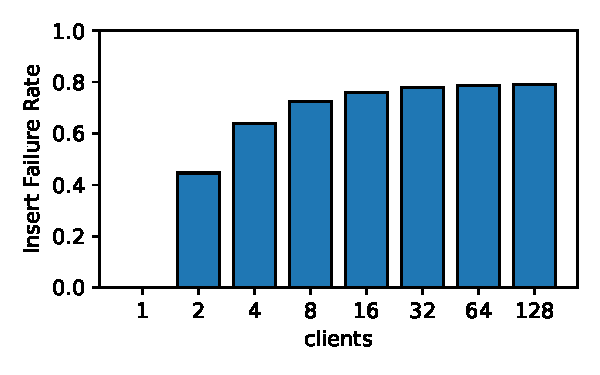
\includegraphics[width=0.99\linewidth]{fig/optimistic_failures.pdf}
        % \label{fig:optimistic_failures}
        % \caption{}
    \end{subfigure}
    \vspace{-1em}
    \caption{
    \textbf{(a)} CX5 RDMA latency vs message size~\cite{rdma-latency}
    \textbf{(b)} ~\todo{make}
    \textbf{(c)} ~\todo{make}
    }
    \label{fig:problems}
\end{figure*}

%concurrent data structures round trips
Concurrent data structure design for remote memory is hard.
Access latency to remote memory is high so round trips per
operation must be minimized to achieve efficiency.
Serialization is particularly hard because there is no
centralized serialization point to guard access to remote
memory. RDMA NIC's provide atomic verbs such as
compare-and-swap (CAS), but these are by no means a silver
bullet.  Each atomic request takes a round trip from client
to server to execute. In the best case lock/unlock requires
two round trips, if multiple locks are required, or locks
are contested the number of round trips increases.

%cpu locking vs rdma
In traditional key value stores (Memcached~\cite{memcached})
the CPU coordinates table access for read, write, and lock
instructions. In contrast RDMA based Key-value
stores~\cite{herd,erpc,pilaf} use a mixture of one-sided (no
cpu) and two-sided (cpu involved) verbs to alleviate the CPU
bottleneck. Reads are typically one sided to bypass the CPU
bottleneck~\cite{pilaf,cell} while writes are typically two
sided so memory-side CPU can orchestrate serialized
operations (e.g. locking) with main memory access latency
(50-100ns).  These small access times keep critical sections
small for CPU based locking, and dramatically increase them
for one-sided RDMA based locking schemes~\cite{clover,
sherman}.

\textbf{Caching:} Modifying a remote data structure requires
clients to have synchronized caches. The cache can either be
accumulated per operation and be discarded or persist across
operations.  Accumulating a cache per operation is slow,
clients must aquire locks, read, then release potentially
many times to complete an operation if the locks are fine
grained. Alternatively clients can persist a cache across
requests in the hope that it will be valid for future
operations.  Clover (a remote memory key value store) caches
pointers to values on clients to enable fast reads when
values are looked up multiple times~\cite{clover}.
Optimistic caching threads a fine line as issuing optimistic
operations which commonly fail may be worse than acquiring
the correct locks.  An ideal caching strategy would enable
clients to succeed in their operations frequently while not
requiring much overhead to maintain. 



%cuckoo hashing optimistic vs locks
\textbf{Critical Sections:} Consider executing an insert
into a concurrent cuckoo hash stored in remote memory. A
client with a cached index may have little or very stale
information about the state of the hash table. To insert the
client must gather information by reading buckets to compute
a cuckoo path. With concurrent clients this leads to a
chicken and egg problem when acquiring locks vs making
reads.

%% optimistic inserts
A client can perform inserts opportunistically by executing
lockless read to learn about the hash table, calculating a
cuckoo path, and executing a sequence of dependent CAS
operations for each step in the path. This approach is
scalable as its critical section is only the length of a CAS
instruction and is only limited by RDMA atomic operation
throughput~\cite{design-guidelines}. However, Paths can
become invalid as other clients running concurrent inserts
invalidate the paths. Figure~\ref{fig:problems}(a) shows the
path insertion failure rate as the number of concurrent
clients grows. This approach minimizes round trips as
dependent CAS operations can be batched thanks to in order
delivery provided by RDMA reliable connections.
Unfortunately failed inserts require additional round trips
to both fix the state of the table, and retry the
insert.\sg{Further - Issuing CAS as a batch leads to complex
path failure cases such a single element in the path failing
while others further down the path succeed. Assesing and
fixing such insertion failures without locks is very hard.}

% lock based inserts
Alternatively to get synchronized information the client can
lock the table, then issue reads. However acquiring locks
without knowledge of the table is hard. A global lock
ensures that all reads are synchronized, but bottlenecks
hash table throughput. Alternatively per bucket locks
enable high throughput but calculating which buckets to lock
requires knowledge of the table. A long cuckoo path may
require locking many buckets and many round trips to gather
information about the hash table.
%%
An ideal protocol would enable clients to perform inserts
without bottlenecks the insert performance of the hash
table, while requiring the fewest round trips to construct
and execute the cuckoo path.

% First, acquiring a lock means a round trip. If the table has
% a single lock, then a client is guaranteed to be able to
% gather all the locks it requires in a single round trip.
% However a single lock does not scale as only a single writer
% can write at a time. This matter is made worse by the fact
% that the critical section of the lock is larger in remote
% memory. Breaking the table up into subtables each with it's
% own lock has it's own problems. An insertion with a long
% path will potentially need to acquire many locks. Each of
% which requires a round trip. Therefore using fine grained
% locking increases the tables scalability but increases it's
% base case insertion time.

\textbf{Read Optimization:} Most data center workloads are
read heavy, therefore read operations should be the most
highly optimized~\cite{datacenter-workloads,facebook-memcached}. Prior
approaches such as RACE require two RDMA round trips per
read. The first is a hash index lookup, the second round
trip reads the actual key-value block. RACE must perform two
round trips because entries in the hash index are limited to
64 bits (CAS width). This is commonly not enough to store
both key and value so RACE can not inline both keys and
values in the index structure. Clover~\cite{clover} enables
single round trips reads. However under contention Clovers
reads require pointer chasing which is known to be expensive
due to each pointer resolution requiring a round
trip~\cite{clio,clover,pointer-chaising}. Ideally we would
be able to ensure that reads complete in a single round
trip.

\textbf{Duplicate Keys:} Clients may issue concurrent
inserts for the same key, given that keys may occupy
multiple location detecting and dealing with duplicate keys
is tricky while maintaining high performance. RACE requires
an extra round trip after each insert to check if a
duplicate key was inserted simultaneously~\cite{race}. An
ideal algorithm would prevent key duplication without
requiring additional overheads.


\section{Design}
\label{sec:design}

\subsection{Locality Hashing}
\begin{figure*}[t]
    \centering
    \begin{subfigure}{0.3\linewidth}
        \begin{align*}
            L_1 &= h_1(k) \\
            L_2 &= L_1 + h_2(k) \% f^{f + log_2(h_3(k))}
        \end{align*}
        % \caption{}
        \label{fig:hash_factor}
    \end{subfigure}
    \begin{subfigure}{0.3\linewidth}
        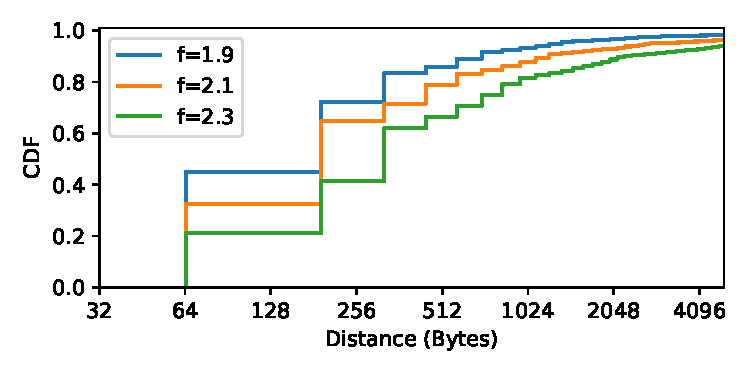
\includegraphics[width=0.99\linewidth]{fig/hash_factor.pdf}
        \label{fig:hash_factor}
        % \caption{}
    \end{subfigure}
    \begin{subfigure}{0.3\linewidth}
        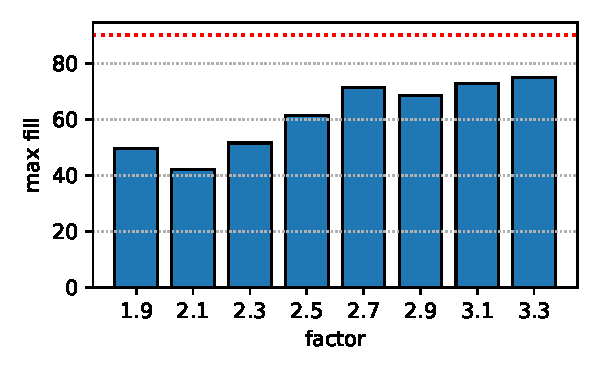
\includegraphics[width=0.99\linewidth]{fig/hash_fill.pdf}
        \label{fig:hash_fill}
        % \caption{}
    \end{subfigure}.
    \vspace{-1em}
    \caption{
    \textbf{(a)} Dependent hashing for factor $f$.
    \textbf{(b)} CDF of distances between cuckoo locations dependent hashing on different exponential factors.
    \textbf{(c)} Exponential factor relation to max fill in cuckoo hash.
    }
    \label{fig:locality-hashing}

\end{figure*}


\begin{figure*}[t]
    \centering
    \begin{subfigure}{0.3\linewidth}
        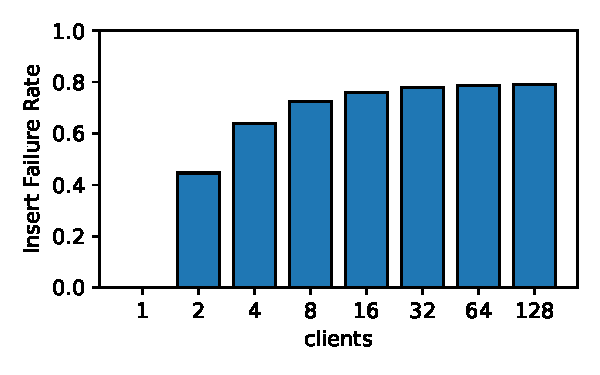
\includegraphics[width=0.99\linewidth]{fig/optimistic_failures.pdf}
        % \label{fig:optimistic_failures}
        % \caption{}
    \end{subfigure}
    \begin{subfigure}{0.3\linewidth}
        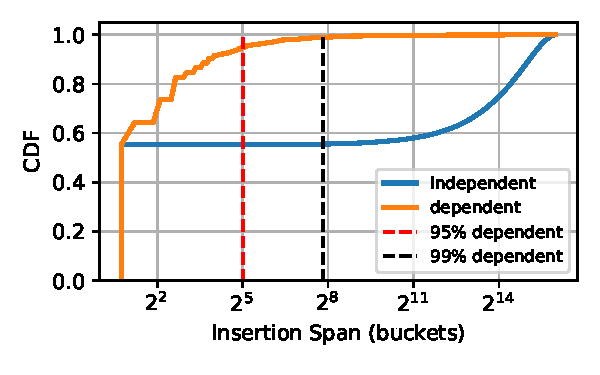
\includegraphics[width=0.99\linewidth]{fig/insertion_span.pdf}
        \label{fig:insertion_span}
        % \caption{}
    \end{subfigure}.
    \begin{subfigure}{0.3\linewidth}
        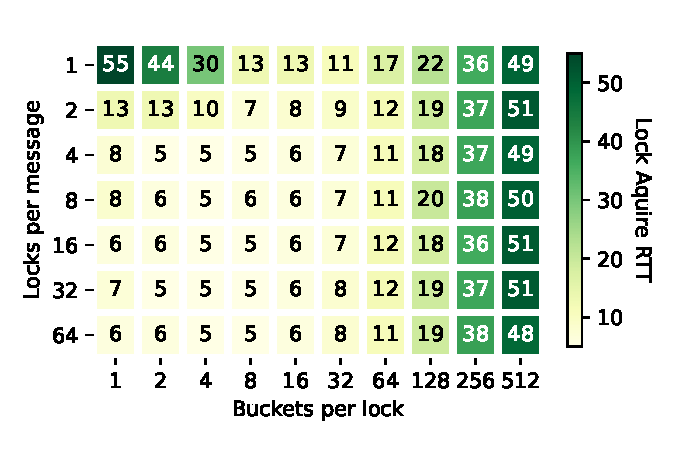
\includegraphics[width=0.99\linewidth]{fig/buckets_per_lock_vs_locks_per_message.pdf}
        \label{fig:tbd}
        % \caption{}
    \end{subfigure}.
    \vspace{-1em}
    \caption{
    \textbf{(a)} Failure rate of optimistic cuckoo insertions.
    \textbf{(b)} CDF of cuckoo spans for dependent and independent hashing. A cuckoo span is the distance between the smallest and largest index in a cuckoo path.
    \textbf{(c)} Round trips (99th percentile) required per insert while filling a table to 100\% while varying the lock per message, and buckets per lock. (\todo{subtract one from each current values include unlocks})
    }
    \label{fig:rdma}

\end{figure*}


Both cuckoo~\cite{cuckoo} and hopscotch~\cite{hopscotch}
hashes are optimized for reads. Cuckoo hashing ensures
constant time reads, while hopscotch hashing ensures that a
read is within a bounded range of it's hash index. Both of
these properties have been noticed by the RDMA key-value
store, and far memory communities for their fast
reads~\cite{memc3,cuckoo-improvements,pilaf,farm}.

Our approach aims to combine the bounded reads of cuckoo
hashing, with the locality properties of hopscotch hashing.
To do so we bound the distance between cuckoo hash
locations. Figure~\ref{fig:rdma}(a) shows the tradeoff
between message size and latency for a ConnectX-5 RDMA NIC.
The latency of small messages (2-128 Bytes) are nearly
identical, and the size of a message must be larger than 1K
before it's latency is 2x that of a small message. Bandwidth
is increasingly available in modern networks with 800Gbps on
the horizon, we tradeoff bandwidth for latency by opting for
larger single messages and fewer round trips. In essence we
make large sloppy reads, and leave it to the client to
reconstruct a result.

Traditional cuckoo hashing calls for two independent hash
functions. We instead make our two hash functions
\textit{dependent}. The first hash function determines the
location a key will be hashed to. The second hash function
determines the maximum distance the second value can have
from the first. A third hash function determines a random
location between the first location, and the bound imposed
by the second. Figure~\ref{fig:locality-hashing}(a) shows
the formula for our dependent hashing function.

A strawman implementation of locality based hashing would
use the first hash function to find a location, and the
second to find a random location within a fixed bound. This
approach quickly leads to failed insertions. Due to the
birthday paradox the probability of a collision is high, and
on large tables the probability that one region of the hash
table will become full, and have not viable path to an open
slot is high. ~\todo{Insert a figure of one of my failed
insertion experiments on a big table}.

Rather than use a static bound we use a dynamic logarithmic
bound with a third hash function. The bound set by the
third hash function is determine by counting the suffix
zeros of the resultant hash and rasing it by an exponential
factor. In the common case the bound is small, but on an
exponentially decrease rate some pairs of values are spaced
far apart. This design enables some pairs to act
as~\textit{waypoints} to other regions of the table. This
method, paired with associative in the cuckoo hash enables
high fill rates while keeping the region of the table any
given key can inhabit small.

The tradeoff between the exponential factor and the mean
distance is fill factor.
Figure~\ref{fig:locality-hashing}(b) illustrates how
increasing the exponential factor shifts the distribution of
distances between cuckoo hash locations.
Figure~\ref{fig:locality-hashing}(c) shows how these same
factors effect the max fill rate of the table before an item
cannot be inserted.


\subsection{Locking}

Traditional wisdom would suggest that because cuckoo hashing
can have long insertion paths it is a poor candidate for
remote memory. Augmenting an insertion path requires making
many modifications to the hash table. There are two
approaches for making path modifications. The first is to
perform a set of compare and swap modification which migrate
an open slot down a path to a location where the new value
is inserted. In this case the client acquires no locks,
however it has no guarantee that it's insertion path with
remain valid as concurrent processes can modify the hash
table with insertions of their own. In this case the client
can opportunistically attempt an insertion path using its
cached information about the table. This strategy has the
potential to fail frequently, and the requires potentially
many reads to be issued for the client to keep it's path
information up to date. ~\todo{insert a plot which shows
path lengths and failure rates from the cukoo approach with
no batching.}

Alternatively a client can aquire locks for the table. Locks
typically have poor performance for disaggregated algorithms
because each lock and unlock operation requires a round
trip. This means that any locking algorithm will have a lock
acquisition phase in which all required locks are collected,
followed by a critical section in which the operations are
executed, and a lock release stage. Using a course grained
locks this approach leads to throughput bottlenecks as it
does not scale with the number of clients. However course
grained locks have the advantage that there are few locks to
aquire, therefore a lock acquisition and release algorithm
takes less round trips. A typical lock acquisition policy
works by acquiring locks in a predefined incremental order to
avoid deadlock. The tradeoff between fine grained and course
locking is clear - fine grained locking allows higher
degrees of parallelism and throughput, while adding higher
latency due to a more complex lock aquire and release stage.
Course locking has lower latency aquire and release, but
limits throughput as many clients will contest the same
locks.

Locality hashing enables very efficient locking due to RDMA
masked CAS
operations~\cite{advanced-transport,scalable-locks}. Without
local hashing fine grained locks would be scattered
throughout the hash table. Locality hashing increases the
probability that an insertion path is within a bounded
region of the hash table.  This means that a lock table with
lock locations corresponding to physical locations in the
hash table will be near one another.  
%%
Figure~\ref{fig:rdma}(b) shows the insert span in buckets
using both dependent and independent hashing on a table with
500K entries and 8 entry buckets. A span is calculated as
the distance between the lowest index and the highest index
in a cuckoo path. Past 50\% independent hashing spans a
random range in the table (whenever a displacement occurs on
insert). With dependent locality based hashing 95\% of
inserts span less than 32 buckets, and 99\% less than 256.
%%
RDMA masked CAS operations allow a client to set a 64 bit
mask along with the new, and old values of the cas
operation. This enables the client to atomically set up to
64 contiguous locks. Using these operations clients can
dramatically decrease the number of round trips required to
acquire locks.
%%
Lock granularity effects performance under contention. Using
values from Figure~\ref{fig:rdma}(b) if locks are per bucket
96\% of lock acquisitions can be completed with a single RTT
masked cas. If locks span 4 buckets 99\% of requests can be
completed in a single round trip.
%%
Figure~\ref{fig:rdma}(c) Shows the tradeoff between lock
granularity and the number of locks which can be set in a
single message with locality hashing turned on. The values
reported are the 99th percentile number of round trips
required to acquire locks up to a 90\% fill factor on a
table with 4096 entries and 8 entries per bucket, and 8
concurrent clients. The biggest factor in round trip times
is the number of locks per bucket. On the far right side of
the heatmap (512) only a single global lock exists. Further
the benefit in terms of locks per message falls off quickly
after 1. RDMA masked CAS are beneficial as they allow for
fine grained locking, but setting 3 or more locks per
message has little effect up to 90\% fill rate.

RDMA atomic throughput is
limited~\cite{design-guidelines}~\todo{[swordbox]}. Reducing
the number of atomic messuages also reduces hardware
limitations on the number of operations. Our lock table is
also small in compairision to the true hash table, each lock
is a single bit, and bits can correspond to multiple rows of
the table if we need to save space~\todo{lock size, vs locks
per message figure}. Because we can save lock space due to
masked cas we can also make use device mapped memory for
faster lock aquisition~\cite{sherman}. RDMA device mapped
memory reduces request latency by executing RDMA operations
onto memory which resides on the RDMA NIC. This memory is
highly constrained~\todo{4MB CX5,CX6}, it removes the need
for a PCIe round trip thereby reducing lock aquisition
latency by aproximatly 2x.

\subsection{Table Design}

We design our table with flexibility in mind. Unlike RACE
which is constrained to 64bit table entries due to CAS width
we can store table entires of arbitrary size as table
updates are made with locks and RDMA writes. We support
inlined values in the index for small keys and values to
support single round trip reads. We support a second format
using extents for variable sized values.
Figure~\ref{fig:table-diagram} illustrates our table design.
Each entry includes an extent bit to indicate if the entry
is inlined or stored in an extent.  We make use of device
mapped memory on recent RDMA NIC's (ConnectX-5+) to reduce
locking latency~\cite{sherman} and enable higher throughput.
Device mapped locking avoids an expensive PCIe round trip,
and reduces on NIC blocking when acquiring locks.


\begin{figure}[t]
    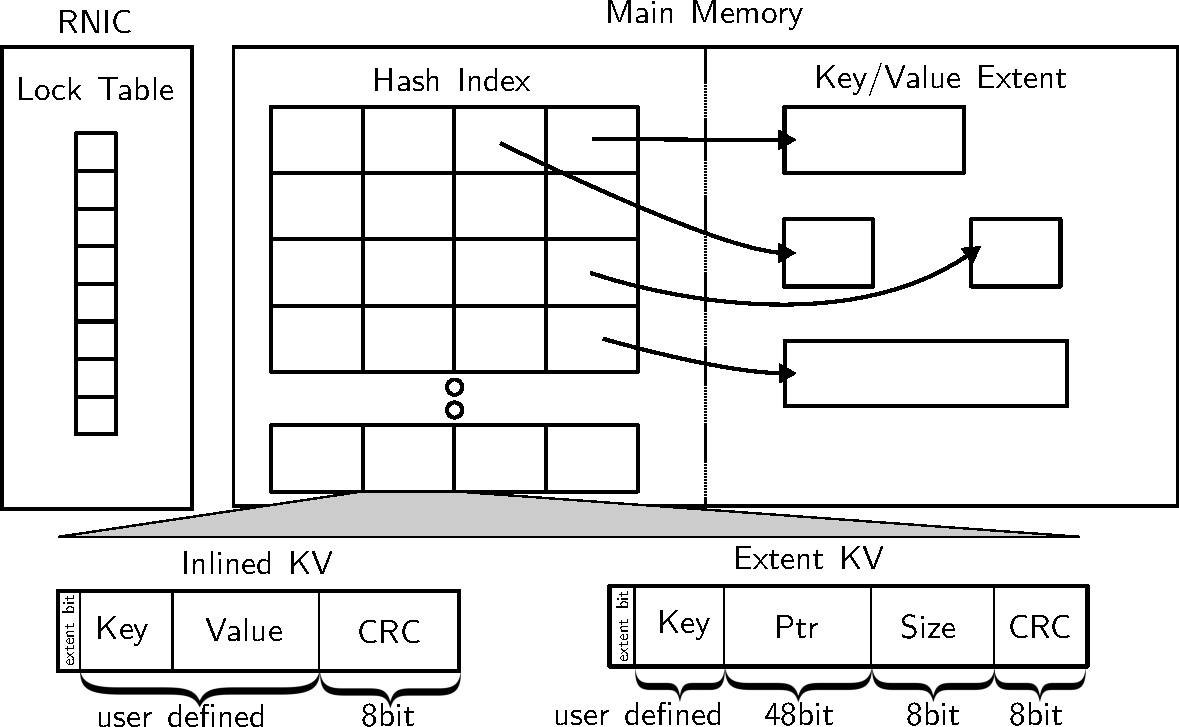
\includegraphics[width=0.99\linewidth]{fig/table-diagram.pdf}
    \caption{Rcuckoo's table design}
    \label{fig:table-diagram}
\end{figure}.


\subsection{Protocol}

Using locks instead of opportunistic concurrency greatly
reduces the round trips required to perform operations.
Insertions into a cuckoo hash require one message for each
entry in the cuckoo path. Executing the insertion
opportunistically with CAS operations enables concurrent
reads, and insertions, but each swap along the path is
blocking as it requires the prior CAS to complete. The round
trips required to perform an opportunistic search is tied to
the length of the cuckoo path. Further as inserts can run
concurrently path insertions can fail. A single failed
insert along the cuckoo path requires the client to stop and
retry it's insert. Alternatively using locks to guard
buckets can guarantee that cuckoo paths can be executed
without failure. Therefore all cuckoo path swaps can be
batched together into a single round trip.

Clients need their caches to be synchronized with the remote
hash table in order to generate correct cuckoo paths. We
batch reads with RDMA masked CAS operations to synchronize
their caches. When a lock request is issued a single read
which spans the range of the lock request is generated. The
read is issued after the lock request, although the two are
batched together. RDMA reliable connections ensure that on a
single QP operations are executed in order. Therefore if the
lock request returns successfully the batched read will
return synchronized values from the hash table which will
remain unmodified while the lock is held.

Clients with synchronized reads can generated cuckoo paths
which are guaranteed to be valid with lock search.
Therefore, all cuckoo path updates can be issued in a single
batch. Further, CAS operations can be swapped with writes.
Writes have higher throughput than CAS, and slightly lower
latency. We add checksums to our table entries to enable
concurrent reads~\cite{pilaf,cell}.  ~\todo{insert RDMA
benchmark for writes and cas.}

Given this propery our protocol for lock aquisition is as
follows. The client performs a search on its local cache for
an insertion path. A set of locks required for the insert
are generated. The locks are broken into a sequence of RDMA
masked CAS operations. Reads which span the range of each
locked bucket are generated alongside the maksed CAS
operations. Clients issue the lock request and the read
behind it. Once the locks are aquired and the reads are
received the clients cache is up to date.

The insertion path the client used to aquire locks may be
invalid after the lock have been aquired. The client
performs a second search for an insertion path only
searching entries from buckets it has locked. If a path
exists the client generates a sequence of write requests,
and unlock requests. The client issues writes and unlocks in
a batch. This read-lock, search, write-unlock pattern along
with locality hashing ensures that in most cases insertions
(as well as deletes and updates) are performed in two round
trips.

Our protocol saves round trips in comparison to RACE, which
uses three round trips in the common case. On inserts RACE
must re-read the hash table to ensure that concurrent CAS
operations did no insert duplicates. With our algorithm we
can simply check for duplicates by reading both insertion
hash locations when acquiring locks. On updates RACE must
read the index, then the data, and then perform the update
as the index is not large enough to store the key. 

RACE requires that each hash table index is 64 bits so it
can be atomically modified by a CAS. Because we use locks
our index can store larger entries containing the key. It
further enables us to store values in the index enabling
single RTT reads. This strategy increase our common case
read size in excahnge for latency~\todo{evaluation section}.
This same pattern is true in RACE for deletes. 
\todo{insert protocol message figure}

\textbf{Key Duplication:} Unlike RACE our algorithm can
prevent duplicate keys easily on insert. Cuckoo hashing
inserts to exactly one bucket, which is read during the lock
acquisition phase. If a duplicate key is found the client
can abort. If the bucket is full, a duplicate key may exist
in it's alternative bucket. Our clients issue a read to the
inserted keys alternative bucket during lock acquisition. If
the lock returns successfully and no duplicate exists in
either bucket then no duplicates exist as the successful
lock ensures that no other client is currently moving the
key to another location as part of a concurrent insert.


\textbf{Reading:} For inlined reads client complete reads in
a single round trip. We trade off latency for bandwidth by
issuing a single read rather than two for reads which span a
small enough range to fit into a single message. This
increases bandwidth consumption per read, but drops the
overall processing required by the memory NIC. Our reading
threshold is configurable. We chose to read up to 512 bytes
in a single read as this covers over 50\% of all reads for
64 bit table entries~\ref{fig:locality-hashing}.

\subsection{Search}
Cuckoo hashing insert traditionally uses random
replacement~\cite{cuckoo}. Random replacement requires
little computation, however at high fill rates it leads to
long cuckoo paths which require many locks, and reduce
concurrent throughput. BFS search finds the shortest path
and has been demonstrated to increase system throughput with
fine grained locking~\cite{algorithmic-improvements}.

BFS search is computationally intensive. Locality based
hashing enables us to leverage more efficient search
strategies. Because locality hashing increases the
probability that a cuckoo hashing location is close we can
use an informed search algorithm to find open slots close to
bucket a key hashes to. 

In the case of BFS the target bucket is unknown, therefore
all paths must be explored. We use A* search, an algorithm
which takes a goal location, and a distance heuristic as
input. A* is known to find shortest paths in much better
average case times than BFS. A* requires two additional
inputs, a distance heuristic and a goal location.

\textbf{goal location}: Locality hashing increases the
probability that an open slot near the insertion target
location can terminate a cuckoo path. Our algorithm collects
open slots near the original hash location as candidate goal
locations. By default we set the number of candidate goal
locations to 5. Gloal locations are collected by starting at
the $h_1(k)$ location and iterating through the hash
table both forward and backwards through the table one index
at a time. Buckets with open slots are added to the
candidate list until the limit is reached. \todo{I could
improve this search time by tracking the list of open
buckets and using binary search on them.}.

\textbf{Search Heuristic}: A* requires a heuristic for
distance which is a strict underestimate of the true
distance to a goal. A typical heuristic for search is the
euclidean distance between two points. A * guarantees that
if the search heuristic is a strict underestimate of the
true distance to the goal then the path found will be the
shortest path. In our case we use the distance between a
goal state and a current state is unknown as the distance
between any two buckets is the result of our locality
hashing function which has no upper bound. However we can
estimate the distance between two buckets by using the mean
distance of our locality hash function. This approach does
not guarantee that we find the shortest path, however it
does find short paths in the common case, and results in
very short search times.

\section{Implementation} We implement our algorithm in
Python and emulate client based RDMA using a custom built
simulator consisting of 1k lines of python. 

\textbf{Simulator:} Our simulator is event based and does
not emulate network transit time, processing time, or failed
packets. Clients, memory, and switches are modeled as finite
state machines, and the network as FIFO queues. Events are
scheduled randomly, between clients, memory, and the
network. RDMA verbs are modeled as function pointers with
arguments passed by the client.

\textbf{Rcuckoo:} Cuckoo is implemented in 1.2k lines of
python. A* is implemented by hand, with the use of python's
standard heap library for priority queuing. Clients store
complete copies of the remote hash table index locally, and
none of the extent in simulation. In practice for better
resource utilization cached pages of the index could be
released using LRU. Our current implementation does not
include extents, all table accesses are inlined.

\textbf{RACE:} We implement RACE~\cite{race} to the best of
our abilities as no publicly available implementation is
available. We only model the RACE index. In cases where
blocking calls are made to RACE's extent we assume they
succeed and simply reissue a read to the index to model the
round trip incurred by the extent lookup. We model RACE's
blocking behavior exactly in this way. We reached out to
RACE's authors to check our implementation's correctness and
were able to correlate our fill factor results with theirs.

\section{Evaluation}
\label{sec:eval}

\begin{figure*}[ht]
    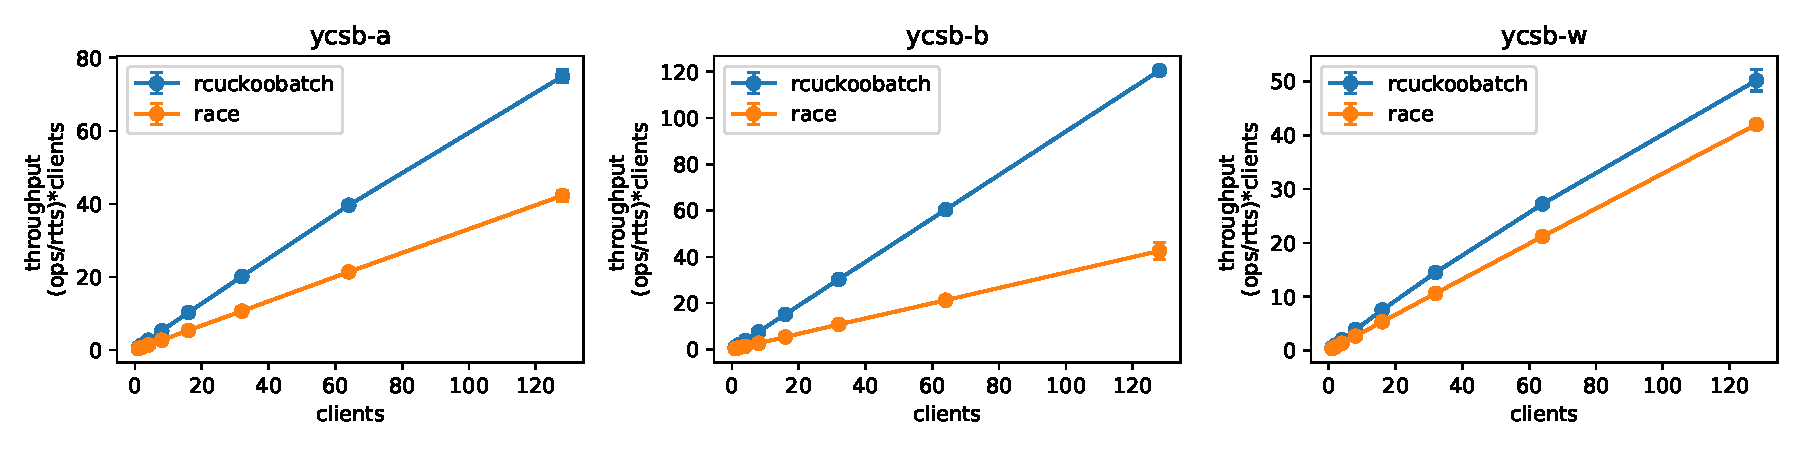
\includegraphics[width=0.99\linewidth]{fig/hero_ycsb_throughput.pdf}
    \caption{race vs rcuckoo simulated throughput}
    \label{fig:ycsb_throughput}
\end{figure*}

\begin{figure*}[ht]
    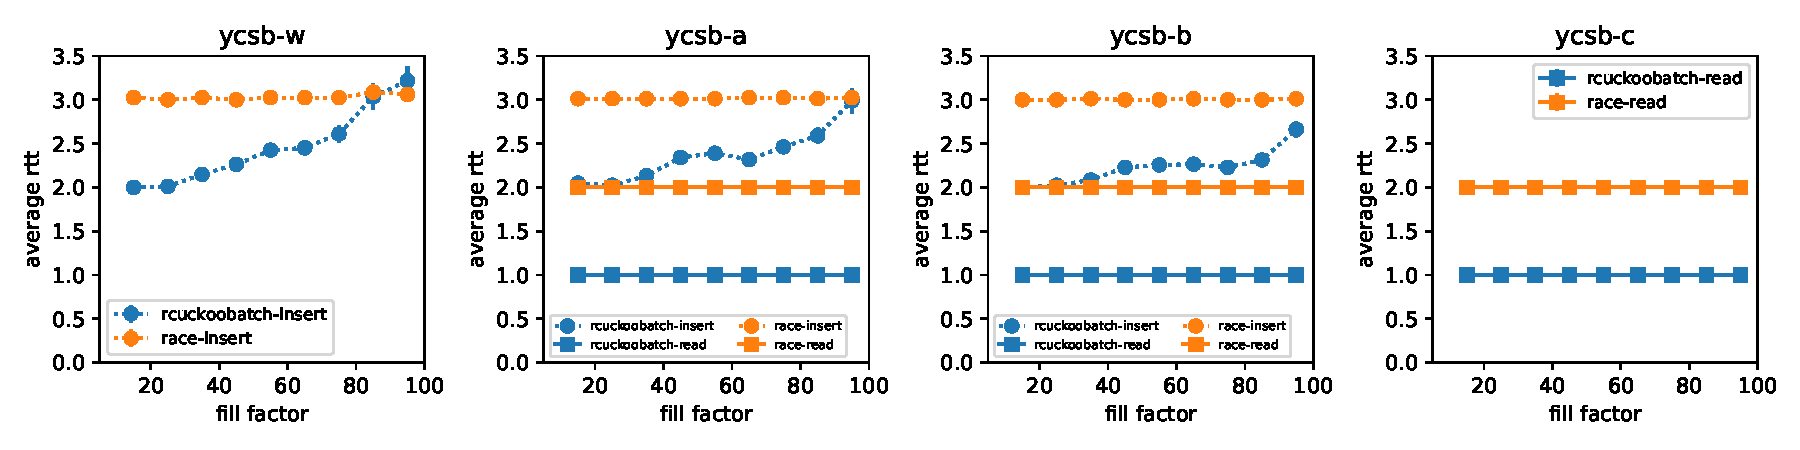
\includegraphics[width=0.99\linewidth]{fig/hero_ycsb_fill_latency.pdf}
    \caption{race vs rcuckoo workload fill latency}
    \label{fig:ycsb_fill_latency}
\end{figure*}

\begin{figure}[ht]
    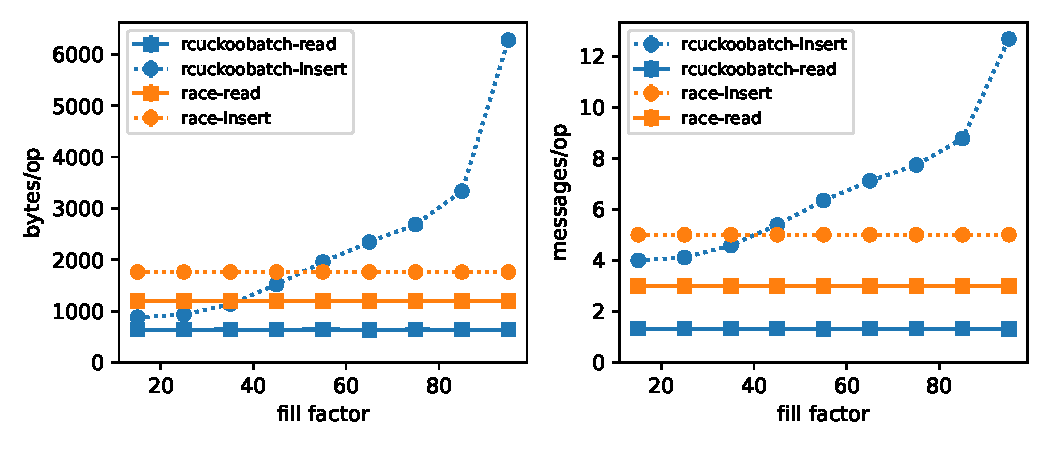
\includegraphics[width=0.99\linewidth]{fig/hero_ycsb_fill_ops_bw.pdf}
    \caption{YCSB-A workload messages and bandwidth per operation as a function of fill factor}
    \label{fig:ycsb_fill_latency}
\end{figure}

\begin{figure}[ht]
    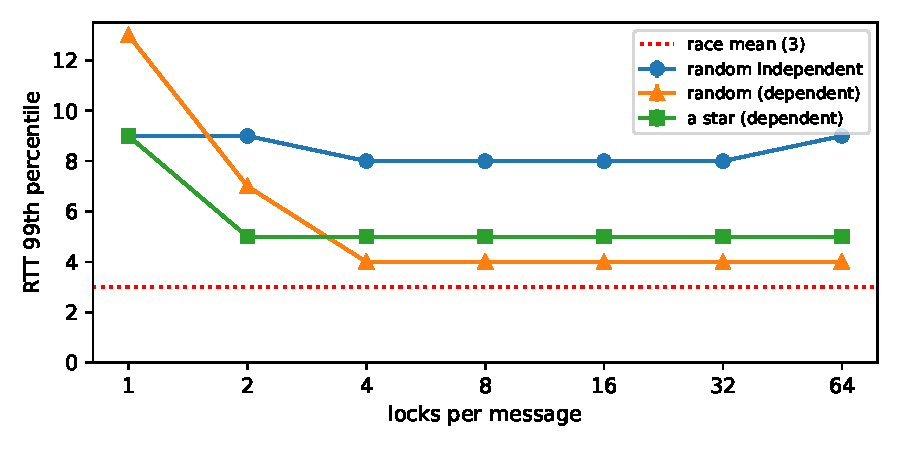
\includegraphics[width=0.99\linewidth]{fig/search_dependence.pdf}

    \caption{Round trips per insert operation compared
    across search functions and hash functions. Dependent
    hash functions with A* have the shortest search times.}

    \label{fig:search_dependence}
\end{figure}

Our evaluation is run entirely in simulation. The goal of
our evaluation is to demonstrate the practicality of Rcuckoo
by showing by proxy that it supports low latency and high
throughput operations. We measure blocking round trip's as a
proxy for latency to measure throughput we normalize the
number of simulation steps each client runs for before
filling the table. Steps do not correlate directly to time,
however the less time a client spends blocking, and the
fewer steps required to complete an operation are a proxy
for real system throughput.

All of our evaluations are carried out on hash tables with
buckets of size 8, and key-value pairs with 32bit keys and
16bit values. On hash tables with 1 million entries.

\subsection{System Breakdown}

Breakdown of insertion performance 

\subsection{System Performance}


Figure~\ref{fig:ycsb_throughput} shows the throughput of race vs rcuckoo for YCSB workloads.

YCSB-A, YCSB-B, and YCSB-C, YCSB-W, for latency.
YCSB-A, YCSB-B, and YCSB-C, YCSB-W, for throughput.
YCSB-A, YCSB-B, and YCSB-C, YCSB-W, for operations per second
YCSB-a, YCSB-b, and YCSB-c, YCSB-w, for bandwidth.



\subsection{Search Performance:}

\textbf{Hashing Algoritms:} Rcuckoo hashing requires
executing many hash compuations. We evalute our A* search
alorithm abolute performacne on various hash functions and
show how this values effect our overall fill factors.

\textbf{A* search vs BFS:} We compare the performance of A*
vs BFS for locally computed insertions. A* performance
directly effects system throughput as this algorithm is run
twice on every insert.


\section{Conclusion}
\label{sec:conclusion}
